\documentclass[12pt,letterpaper]{article}

%\usepackage{common}
\usepackage{amsmath}
\usepackage{amssymb}
\usepackage{mathtools}
\usepackage{nicematrix}
\usepackage{algorithm}
\usepackage{algpseudocode}
\usepackage{tcolorbox}
\usepackage{nicefrac}
\usepackage{enumerate}
\tcbuselibrary{theorems}

\usepackage{hyperref}

\usepackage{parskip}
%\setlength{\parskip}{\baselineskip}
%\setlength{\parindent}{0pt}

\usepackage{tikz}
\usepackage{pgfplots}
%\usepgfplotslibrary{external}
%\tikzexternalize
 \definecolor{sylveonblue}{HTML}{3d93ff}
 \definecolor{sylveonpink}{HTML}{c27386}
 \definecolor{sylveonteal}{HTML}{859ee1}

\usepackage{pxpic} %Silly

\renewcommand{\algorithmicrequire}{\textbf{Input:}}
\renewcommand{\algorithmicensure}{\textbf{Output:}}

\newcommand{\skipline}{\vspace{\baselineskip}}
\newcommand{\dis}{\displaystyle}
\newcommand{\noin}{\noindent}

\newcommand{\R}{\mathbb{R}}
\newcommand{\C}{\mathbb{C}}
\newcommand{\mt}[1]{\text{#1}}
\newcommand{\tr}{\mathrm{Trace}}
\newcommand{\Tr}{\mathrm{Trace}}
\newcommand{\Ker}{\mathrm{Ker}}
\newcommand{\dd}{\mathrm{d}}
\newcommand{\fl}{\mathrm{fl}}
\newcommand{\bigO}{\mathcal{O}}

\DeclarePairedDelimiter\abs{\lvert}{\rvert}

\newtcbtheorem[number within=section]{theo}{Theorem}{colback=green!5,colframe=green!35!black,fonttitle=\bfseries}{th}
\newtcbtheorem[number within=section]{coro}{Corollarly}{colback=green!5,colframe=green!35!black,fonttitle=\bfseries}{th}
\newtcbtheorem[number within=section]{lemma}{Lemma}{colback=green!5,colframe=green!35!black,fonttitle=\bfseries}{th}
\newtcbtheorem[number within=section]{defn}{Definition}{colback=red!5,colframe=red!35!black,fonttitle=\bfseries}{th}
\newtcbtheorem[number within=section]{constr}{Construction}{colback=yellow!5,colframe=yellow!35!black,fonttitle=\bfseries}{th}
\newtcbtheorem[number within=section]{algo}{Algorithm}{colback=blue!5,colframe=blue!35!black,fonttitle=\bfseries}{th}
%\newtcbtheorem[number within=section]{lemma}{Lemma}{colback=yellow!5,colframe=yellow!35!black,fonttitle=\bfseries}{th}

\pxpicsetup{
	mode=px,
	colours={
		d=black,
		w=white,
		p=[HTML]{f88ca6},
		l=[HTML]{ffd9e3},
		L=[HTML]{eab4cb},
		b=[HTML]{3d93ff},
		c=[HTML]{6adbfb},
		u=[HTML]{859ee1},
		r=[HTML]{644243},
		g=[HTML]{424244},
		E=[HTML]{48bdff},
		e=[HTML]{bde7fd},
		a=[HTML]{7cbfc5},
		P=[HTML]{d5abc3},
		R=[HTML]{c27386}
	},
	skip=.,
	size=5pt
}

\title{AMSC 460 Root Finding}
\author{Dennis Chunikhin}
\date{\today}

\begin{document}

\maketitle

%\[
%<3
%\]

\skipline\skipline

% The silly
\pxpic{
{.........dd}
{........dppd}
{......ddgppd}
{....ddccgppd........dd}
{...dpbcrgppd......ddppd}
{...dpbccrppd.....dppppd}
{....duruppd.....dpppppd}
{.....ducppd.dd.dppbbpd....d}
{.....dpggggd..dppccpppd..dcdd}
{....drrpppg...gpbcpppd...dcdcd}
{...dppppppg.lpgbbpppd...dbuccd}
{....dpppppg.ppRgggpd....dpbcd}
{...dpppppppggRpp..d...ddgPud}
{....dwpppppppgpl..gddd...Pd}
{....dEwppwwllglwwgPP....dd}
{....dewpwwEElPgggPP..ggd}
{...dlbwwwE.EEwppddddgppd}
{...dllwwweecbwld....dppd}
{....dlwwwacblllgddddupd}
{..dd.ggwwggllgg....lgd}
{.d.g.ppggp.gg...gggPPPd}
{d..g.lpppp.dl.gglllggPPd..ddd}
{d.gPg.lgp..gggllllllgdPPdduccd}
{.ddPPgdpg.gLlllllLllLgdPPuudd}
{...ddd.dPgPwwPdddllLLd.dddd}
{........dPPwwd...dlLd}
{........dggwgd....dpd}
{.........dwwd....dppd}
{.........dppd.....dd}
{........dppd}
{.........dd}
}
 
\newpage

\tableofcontents

\newpage

\section{Nonlinear Optimization: 1D Root-Finding}

We want to find the root of some arbitrary function $f$. That is, given $f : \R \rightarrow \R$, find $x^*$ such that $f(x^*) = 0$.

This is equivalent to optimization since when arbitrary function $g(x^*)$ is at a minimum, its derivative $g'(x^*)=0$.

\subsection{Bisection Method}

\begin{algo}{Bisection Method}
.Suppose we have continuous function $f: \R \rightarrow \R$.

Suppose we have two points $x_l$ and $x_r$ such that $f(x_l)$ and $f(x_r)$ have different signs.

\begin{algorithm}[H]
\caption{Find the root of $f$ using the bisection method.}
\begin{algorithmic}[1]
\Require{$x_l, x_r$}
\Ensure{$x_m^{(k)} \approx x^*$}
\Statex
\Function{root}{$f, x_l, x_r$}
\State Let $x_l^{(k)} = k$-th left point \Comment{$x_l^{(0)} = x_l$}
\State Let $x_r^{(k)} = k$-th right point \Comment{$x_r^{(0)} = x_r$}
\State $x_m^{(k)} = \frac{x_l^{(k)} + x_r^{(k)}}{2}$ \Comment{$k$-th midpoint}
\item[]
\If{$f(x_m^{(k)})$ has the opposite sign as $f(x_l^{(k)})$}
\State $x_r^{(k+1)} = x_m^{(k)}$
\Else
\State $x_l^{(k+1)} = x_m^{(k)}$
\EndIf
\item[]
\State Repeat these steps.
\EndFunction
\end{algorithmic}
\end{algorithm}
\end{algo}

\subsubsection{Bisection Method Convergence}
Since each step we cut the interval $\left\lvert x_l^{(k)} - x_r^{(k)} \right\lvert$ in half, after $k+1$ steps we have:
\begin{equation}
	\left\lvert x_l^{(k)} - x_r^{(k)} \right\lvert \leq \frac{1}{2^{k+1}} \left\lvert x_l - x_r \right\lvert
\end{equation}

Moreover, since the root $x^*$ stays within the interval, the distance between the midpoint (our best guess of the root) and the root is smaller than the interval itself:
\begin{equation}
	\left\lvert x_m^{(k)} - x^* \right\lvert \leq \left\lvert x_l^{(k)} - x_r^{(k)} \right\lvert
\end{equation}

The right hand side is our error (distance between our guess of the root and the actual root). We want the error $\left\lvert x_m^{(k)} - x^* \right\lvert$ to be below some tolerance $\tau$. This is satisfied if:
\begin{align}
	& \left\lvert x_m^{(k)} - x^* \right\lvert
	\leq \left\lvert x_l^{(k)} - x_r^{(k)} \right\lvert
	\leq \frac{1}{2^{k+1}} \left\lvert x_l - x_r \right\lvert
	\leq \tau \\
	\implies & \frac{1}{2^{k+1}} \leq \frac{\tau}{\left\lvert x_l - x_r \right\lvert} \\
	\implies & 2^{k+1} \geq \frac{\left\lvert x_l - x_r \right\lvert}{\tau} \\
	\implies & k+1 \geq \log\left(\frac{\left\lvert x_l - x_r \right\lvert}{\tau}\right) = \log\left(\left\lvert x_l - x_r \right\lvert\right)-\log(\tau) \\
	\implies & k+1 \geq -\log(\tau) \label{eq:bisection_log_ineq} \\
	\implies & k \geq -\log(\tau)
\end{align}
Here $\log$ denotes log base 2.

Note: step \ref{eq:bisection_log_ineq} holds if $\log\left(\left\lvert x_l - x_r \right\lvert\right)$ is positive or much smaller than $-\log(\tau)$. Since we expect the intial interval to be much larger than the tolerance, this is a fair assumption.
Moreover, since the tolerance $\tau$ is a very small positive number, we expect $-\log(\tau) > 0$, and we can thus write $-\log(\tau) = \lvert \log(\tau) \rvert$.

This is a pretty good condition! E.g. if $\tau$ is of the order $10^{-6}$, we would need about $20$ steps.

\begin{theo}{Bisection Method Step Count}
.The number of steps $k$ needed to find the root of an arbitrary function $f$ to within some tolerance $\tau$ using the bisection method is given by:
\begin{equation} \label{eq:bisection_er}
	k \geq \big\lvert \log(\tau) \big\rvert
\end{equation}
\end{theo}

\subsection{Newton's Method}
We have described and derived Newton's method before, but it is worth re-deriving it using linearization via the Taylor series.

We approximate an arbitrary function $f$ around point $x_n$ using its Taylor expansion
\begin{align}
	f(x_n + \delta) &= f(x_n) + f'(x_n) \delta + \bigO(\delta^2) \\
	&\approx f(x_n) + f'(x_n) \delta
\end{align}

Note from me: this still requires the same continuity assumtion for $f$.

We then use this approximation to find the root:
\begin{align}
	& f(x_n) + f'(x_n) \delta = 0 \\
	\implies & \delta = -\frac{f(x_n)}{f'(x_n)}
\end{align}

A step of the Newton's method is then
\begin{align}
	x_{n+1} &= x_n + \delta \\
	&= x_n - \frac{f(x_n)}{f'(x_n)}
\end{align}

\begin{algo}{Newton's Method}
.A step of Newton's method is given by
\begin{equation}
	x_{n+1} = x_n - \frac{f(x_n)}{f'(x_n)}
\end{equation}
\end{algo}


\subsubsection{Newton's Method Convergence}
As before, the error is defined as the distance between our guess of the root $x_n$ and the true root $x^*$. We ask whether the error converges to $0$, and if so how many steps does it take for it to fall below some threshold $\tau$:
\begin{equation}
	\left\lvert x^* - x_n \right\rvert \leq \tau
\end{equation}

Observe that
\begin{equation}
	f(x^*) - f(x_n) = \int_{x_n}^{x^*} f'(t) \dd t
\end{equation}

Since $x^*$ is a root of $f$, $f(x^*) = 0$ by definition. Thus
\begin{equation} \label{eq:newton_conv_1}
	-f(x_n) = \int_{x_n}^{x^*} f'(t) \dd t
\end{equation}

Additionally, consider the constant $f'(x_n)$. Since this is just some constant number,
\begin{equation} \label{eq:newton_conv_2}
	(x^* - x_n) f'(x_n) = \int_{x_n}^{x^*} f'(x_n) \dd t
\end{equation}

Now we subtract equation \ref{eq:newton_conv_2} from equation \ref{eq:newton_conv_1}:
\begin{equation}
	-f(x_n) - (x^* - x_n) f'(x_n) = \int_{x_n}^{x^*} \left[ f'(t) - f'(x_n) \right] \dd t
\end{equation}

Then divide both sides by $f'(x_n)$
\begin{equation}
	-\frac{f(x_n)}{f'(x_n)} - (x^* - x_n) = \frac{1}{f'(x_n)} \int_{x_n}^{x^*} \left[ f'(t) - f'(x_n) \right] \dd t
\end{equation}

Notice that $x_n - \frac{f(x_n)}{f'(x_n)} = x_{n+1}$ in our Newton's rule method. Thus the equation becomes
\begin{equation}
	x_{n+1} - x^* = \frac{1}{f'(x_n)} \int_{x_n}^{x^*} \left[ f'(t) - f'(x_n) \right] \dd t
\end{equation}

The right hand side is exactly the error! We can now introduce absolute value signs to get
\begin{align}
	\left\lvert x_{n+1} - x^* \right\rvert &= \frac{1}{\lvert f'(x_n) \rvert}
	\left\lvert \int_{x_n}^{x^*} \left[ f'(t) - f'(x_n) \right] \dd t \right\rvert \\
	&\leq \frac{1}{\lvert f'(x_n) \rvert} \int_{x_n}^{x^*} \left\lvert f'(t) - f'(x_n) \right\lvert \dd t
	\label{eq:newton_er_eq_pre_assumption}
\end{align}

We must now make some assumptions.

\begin{constr}{Newton's Method Assumptions}
.Given $f$ defined on interval $I$, assume:
\begin{enumerate}[(i)]
	\item $\lvert f'(t) \rvert \geq \rho > 0 \quad \forall t \in I$
	
	\medskip
	That is, $\lvert f'(t) \rvert$ is bounded below by $\rho$ (this assumption allows division by $f'(x_n)$, which is part of Newton's method).
	
	\item $\lvert f'(t_1) - f'(t_2) \rvert \leq \delta \lvert t_1 - t_2 \rvert \quad \forall t_1, t_2 \in I$
	
	\medskip
	Continuity requirement on $f'$.
\end{enumerate}
\end{constr}

Thus if $x_n, t \in I$, then equation \ref{eq:newton_er_eq_pre_assumption} becomes
\begin{align}
	\lvert x_{n+1} - x^* \rvert &\leq \frac{1}{\lvert f'(x_n) \rvert} \int_{x_n}^{x^*} \left\lvert f'(t) - f'(x_n) \right\lvert \dd t \\
	&\leq \frac{1}{\rho} \int_{x_n}^{x^*} \delta \left\lvert t - x_n \right\lvert \dd t \\
	&= \frac{\delta}{\rho} \int_{x_n}^{x^*} \lvert t - x_n \rvert \dd t \\
	&= \frac{\delta}{\rho} \cdot \frac{1}{2} (x^* - x_n)^2 \label{eq:newton_error_integral}
\end{align}

Note that because of the square, the integral evaluates to $\frac{1}{2}(x^* - x_n)^2$ regardless of whether $x^* > x_n$ or $x^n > x^*$ (you can confirm this by evaluating the integral for each of these cases).

Denote the error at step $n$
\begin{equation}
	e_n = \lvert x_n - x^* \rvert
\end{equation}

Equation \ref{eq:newton_error_integral} tells us that
\begin{equation}
	e_{n+1} \leq \frac{\delta}{2\rho} e_n^2
\end{equation}

Denote
\begin{equation}
	\alpha = \frac{\delta}{2\rho}
\end{equation}
For our purposes, $\alpha$ is just some constant.

\begin{theo}{Newton's Method speed of convergence}
.The error in Newton's method follows
\begin{equation} \label{eq:Newton_speed_conv}
	e_{n+1} \leq \alpha e_n^2
\end{equation}
\end{theo}

This gives us the speed of convergence once we are close 

\begin{theo}{For a small enough initial interval, Newton's method converges.}
.We claim without proof that if the interval
\begin{equation}
	\lvert I \rvert \leq \frac{1}{2\alpha}
\end{equation}
then each $x_j \in I$ and
\begin{equation}
	e_{n+1} \leq \frac{1}{2} e_n
\end{equation}
\end{theo}

This implies that
\begin{equation}
	e_n \leq \frac{1}{2} e^{n-1} \leq \cdots \leq \frac{1}{2^n} e_0
\end{equation}

This guarantees that $e_n \rightarrow 0$ as $n \rightarrow \infty$.

Equation \ref{eq:Newton_speed_conv} gives us the speed of convergence once we are close enought to $x^*$:

\begin{theo}{Newton's method error converges double exponentially once we are close enough}
For simplicity let's assume that $\alpha = 1$. Then by equation \ref{eq:Newton_speed_conv}
\begin{equation}
	e_n \leq e_{n-1}^2 \leq \left( e_{n-2}^2 \right)^2 \leq \cdots \leq e_0^{2^n} \quad \text{if } e_0 < 1
\end{equation}
\end{theo}
In the homework we generalize this result for any $\alpha$.

Next we find how many Newton's methods steps are needed to achieve some error tolerance $\tau$--that is so that $e_n \leq \tau$:
\begin{align}
	e_n &\leq \tau \\
	e_0^{2^n} &\leq \tau \\
	\log e_0^{2^n} = 2^n \log e_0 &\leq \log\tau \label{eq:Newton_conv_log}
\end{align}

Since $e_0 < 1$ (from the interval of convergence) and presumably $\tau < 1$, $\log e_0$ and $\log\tau$ are negative, meaning we can rewrite equation \ref{eq:Newton_conv_log} as
\begin{align}
	2^n \lvert \log e_0 \rvert &\geq \lvert \log \tau \rvert \\
	2^n &\geq \frac{\lvert \log \tau \rvert}{\lvert \log e_0 \rvert} \\
	n &\geq \log \frac{\lvert \log \tau \rvert}{\lvert \log e_0 \rvert} \\
	&\quad= \log \lvert \log \tau \rvert - \log \lvert \log e_0 \rvert \label{eq:Newton_n_log_1}
\end{align}
where $\log$ is the logarithm base 2.

Again from the interval condition (theorem 1.3), we will certainly have $e_0 \leq \nicefrac{1}{2}$. This means that $\log e_0 \leq -1$, meaning that $\lvert \log e_0 \rvert \geq 1$. Thus, $\log \lvert e_0 \rvert \geq 0$, which means that equation \ref{eq:Newton_n_log_1} becomes
\begin{align*}
	n &\geq \log \lvert \log \tau \rvert - \log \lvert \log e_0 \rvert \\
	&\geq \log \lvert \log \tau \rvert
\end{align*}

\begin{theo}{Newton's method: number of steps needed to achieve a tolerance grows as $\log \log$}
.If we are close enough to $x^*$ (and the assumptions above still hold, e.g. $\alpha=1$), the number of Newton's method steps $n$ needed to achieve tolerance $\tau$ is bounded by
\begin{equation}
	n \geq \log \lvert \log \tau \rvert
\end{equation}
\end{theo}
As before, in the homework we generalize this resultz for any $\alpha$.

Note that this is a much faster convergence than the bisection method (and is in general a very good convergence)!


\subsection{Rate of Convergence}
This section builds some mechanisms that we use to compare the convergence of algorithms.

\begin{defn}{Rates of Convergence}
.Let $\gamma < 1$ be some constant.
\skipline

If $e_{n+1} \leq \gamma e_n$, we say the algorithm displays \textbf{linear convergence}.

If $e_{n+1} \leq \gamma e_n^2$, we say the algorithm displays \textbf{quadratic convergence}.

If $e_{n+1} \leq \gamma e_n^p$ for $1 < p < 2$, we say the algorithm displays \textbf{superlinear convergence}. We call $p$ the \textbf{rate of convergence}.
\end{defn}

Bisection method has linear convergence.

Newton's method has quadratic convergence.

As we will see in the next section, the secant method has superlinear convergence. Moreover, the rate of convergence for the secant method is $p = \frac{1 + \sqrt{5}}{2}$, the golden ratio!

\newpage
\subsection{Secant Method}

\begin{tikzpicture}

\end{tikzpicture}

\pgfmathsetmacro{\pa}{0.82}
\pgfmathsetmacro{\pb}{0.96}
\begin{center}
\begin{tikzpicture}[declare function={
	f(\x) = (\x-0.1)*(9*\x^2-13.5*\x+5.3);
	f_prime(\x) = (9*\x^2-13.5*\x+5.3) + (\x-0.1)*(18*\x-13.5);
	f_tan(\x) = f_prime(\pa)*(x-\pa) + f(\pa);
	g(\x) = (f(\pb)-f(\pa))/(\pb-\pa)*(x-\pb)+f(\pb);
}, scale=1]
\begin{axis}[axis x line=center, axis y line=none, xtick={\pa, \pb}, xticklabels={$x_n$, $x_{n-1}$}, ytick={0}]
	\addplot[color=sylveonblue, domain=0:1, samples=100, thick] {f(x)};
	\addplot[color=sylveonblue, mark=*, only marks, samples at={0.1}] {f(x)} node[pin=-50:{$x^*$}]{};
	\addplot[color=sylveonblue, mark=*, only marks, samples at={\pb}] {f(x)};
	\addplot[color=sylveonblue, mark=*, only marks, samples at={\pa}] {f(x)};
	
	\addplot[dashed] coordinates{(\pb, 0)(\pb, f(\pb)};
	\addplot[dashed] coordinates{(\pa, 0)(\pa, f(\pa)};
	
	\addplot[color=teal, domain=0.67:0.995, thick] {g(x)};
	\addplot[color=teal, mark=*] coordinates{(-f(\pa)*(\pb-\pa)/(f(\pb)-f(\pa)) + \pa, 0)}
		node[pin={[pin distance=1.2em]-90:{$x_{n+1}$ Secant method}}]{};
	
	\addplot[color=sylveonpink, domain=0.5:0.995, thick] {f_tan(x)};
	\addplot[color=sylveonpink, mark=*] coordinates{(-f(\pa)/f_prime(\pa) + \pa, 0)}
		node[pin={[pin distance=4em]93:{$x_{n+1}$\ Newton's method}}]{};
\end{axis}
\end{tikzpicture}
\end{center}

The idea behind the Secant method is to approximate the derivative of the function $f$ using the slope between our last and current guess as illustrated above. The advantage of this is lower cost--that is, only 1 function evaluation is needed each step.

The equation of the secant line is:
\begin{equation} \label{eq:secant_line}
	\frac{y - f(x_n)}{x - x_n} = \frac{f(x_n) - f(x_{n-1})}{x_n - x_{n-1}}
\end{equation}

We want to solve for $x=x_{n+1}$ such that $y=0$, so we plug these values into equation \ref{eq:secant_line} and solve for $x_{n+1}$:
\begin{align}
	& \frac{0 - f(x_n)}{x_{n+1} - x_n} = \frac{f(x_n) - f(x_{n-1})}{x_n - x_{n-1}} \\
	\implies & x_{n+1} = x_n - f(x_n) \frac{x_n - x_{n-1}}{f(x_n) - f(x_{n-1})}
\end{align}

\begin{algo}{Secant Method}
.A step of the secant method is given by
\begin{equation}
	x_{n+1} = x_n - \frac{x_n - x_{n-1}}{f(x_n) - f(x_{n-1})} f(x_n)
\end{equation}

The advantage of this over Newton's method is that only one function evaluation is needed per step (that is, you do not need to evaluate $f'(x_n)$).
\end{algo}

\begin{theo}{Secant method rate of convergence is superlinear}
.The error in the secant method follows
\begin{equation}
	e_{n+1} \leq \alpha e_n^p
\end{equation}
where $p = \frac{1 + \sqrt{5}}{2}$ is the golden ratio.
\end{theo}

The professor states this without proof in the notes. The error analysis is a bit more involved but not inaccessible; I found a good writeup here: \url{https://www.math.drexel.edu/~tolya/300_secant.pdf}.

\subsubsection{Cost}
We find the number of steps $n$ needed to achieve an error below a given tolerance: $e_n \leq \tau$. To simplify analysis, let's assume $\alpha = 1$. Then
\begin{align}
	e_n \leq e_{n-1}^p \leq (e_{n-2}^p)^p \leq \cdots \leq e_0^{p^n} \leq \tau
\end{align}

We take the logarithm of both sides:
\begin{align}
	\log e_0^{p^n} &\leq \log \tau \\
	p^n \log e_0 &\leq \log \tau
\end{align}

Assuming $e_0 < 1, \tau < 1$, both of the logarithm are negative, meaning that we can rewrite the expression as
\begin{align}
	- p^n \log e_0 &\geq -\log \tau \\
	p^n \lvert \log e_0 \rvert &\geq \lvert \log \tau \rvert \\
	p^n &\geq \frac{\lvert \log \tau \rvert}{\lvert \log e_0 \rvert}
\end{align}

Take the logarithm again:
\begin{align}
	n \log p &\geq \log \frac{\lvert \log \tau \rvert}{\lvert \log e_0 \rvert} \\
	&= \log \lvert \log \tau \rvert - \log \lvert \log e_0 \rvert \\
	&\geq \log \lvert \log \tau \rvert
\end{align}

For comparison with Newton's method, $\log$ still means the logarithm base 2.

\begin{theo}{Secant method is cheaper than Newton's method}
.To achieve an error below tolerance $\tau$ (with the assumptions from above) the number of steps $n$ the secant method requires is bounded by
\begin{equation}
	n \geq \frac{\log \lvert \log \tau \lvert}{\log p} \approx \frac{\log \lvert \log \tau \lvert}{0.696}
	\approx 1.44 \log \lvert \log \tau \lvert
\end{equation}

where $\log$ is the logarithm base 2.

Thus Newton's method requires $2 n_{\text{newt}}$ function evaluations, while the secant method requires only about $1.44 n_{\text{newt}}$. Thus the secant method is cheaper.
\end{theo}

\section{Nonlinear Optimization: Roots of Multi-Valued Functions of Multiple Variables}
Suppose we have a function $f : \R^n \rightarrow \R^n$. We are seeking $x^*$ such that
\begin{equation}
f(x^*) = \mathbf{0} = \begin{pmatrix}
	0 \\ \vdots \\ 0
\end{pmatrix}
\end{equation}

\subsection{Multivariate Newton's Method}
We derive Newton's method again using Taylor series.

We can describe the multivariate function as a system of equations:
\begin{equation}
f(x) = \begin{pmatrix}
	f_1(x) \\ f_2(x) \\ \vdots \\ f_n(x)
\end{pmatrix}
\end{equation}
where each $f_i : \R^n \rightarrow \R$.

Consider the Taylor series for a given $f_i$:
\begin{align}
	f_i(x_k + \delta) = f_i(x_k) + (\nabla f_i)(x_k)^T \delta + O(\lVert \delta \rVert^2)
\end{align}

Thus, for the entire function
\begin{align} \label{eq:Newton_multi_taylor}
f(x_k + \delta) = f(x_k) + \begin{pmatrix}
	\nabla f_1(x_k)^T \\
	\nabla f_2(x_k)^T \\
	\vdots \\
	\nabla f_n(x_k)^T
\end{pmatrix} \delta + O(\lVert \delta \rVert^2)
\end{align}

The $n \times n$ matrix formed by the gradients is called the Jacobian matrix.

\begin{defn}{Jacobian matrix}
.Given $f : \R^n \rightarrow \R^n$, the Jacobian matrix is
\begin{equation}
J_f(x) = \begin{pmatrix}
	\nabla f_1(x)^T \\
	\nabla f_2(x)^T \\
	\vdots \\
	\nabla f_n(x)^T
\end{pmatrix} =
\begin{pmatrix}
	\frac{\partial f_1}{\partial x_1} & \frac{\partial f_1}{\partial x_2} & \cdots & \frac{\partial f_1}{\partial x_n} \\
	\frac{\partial f_2}{\partial x_1} & \frac{\partial f_2}{\partial x_2} & \cdots & \frac{\partial f_2}{\partial x_n} \\
	\vdots & \vdots & \ddots & \vdots \\
	\frac{\partial f_n}{\partial x_1} & \frac{\partial f_n}{\partial x_2} & \cdots & \frac{\partial f_n}{\partial x_n}
\end{pmatrix}
\end{equation}
all evaluated at $x$.

Think of the Jacobian as our multivariate ``derivative''.
\end{defn}

Newton's method approximates the root using the linear Taylor series approximation obtained from equation \ref{eq:Newton_multi_taylor}:
\begin{equation}
	f(x_k) + J_f(x_k) \delta = 0
\end{equation}

Hence to get $\delta$ we need to solve the equation
\begin{equation}
	J_f(x_k) \delta = -f(x_k)
\end{equation}

\begin{algo}{Multivariate Newton's method}
.Given function $f : \R^n \rightarrow \R^n$, to get the next estimate of the root using the multivariate Newton's method we need to solve the system of equations
\begin{equation}
J_f(x_n) \delta = -f(x_n)
\end{equation}

Then
\begin{equation}
	x_{n+1} = x_n + \delta
\end{equation}

This statement makes the most sense computationally, but we can also write it more concisely mathematically as
\begin{equation}
	x_{n+1} = x_k - J_f(x_k)^{-1} f(x_k)
\end{equation}
\end{algo}

\subsubsection{Cost and Convergence}
Note that computing the Jacobian matrix $J(x_k)$ can possibly be expensive in and of itself.

Additionally, the cost of solving the system is approximately $\frac{1}{3}n^3$ for Gaussian elimination.

We also state the conditions for the convergence of the multivariate Newton's method without proof

\begin{constr}{Multivariate Newton's method converges if the Jacobian is continuous bounded from below.}
.Given $f : \R^n \rightarrow \R^n$ defined in a ball $B$, Newton's method is guaranteed to converge if:

\begin{enumerate}[(i)]
	\item $\lVert J_f(x) - J_f(y) \rVert \leq \gamma \lVert x - y \rVert \quad \forall x, y \in B$
	
	\medskip
	This is the continuity of $J_f$, and is analogous to the continuity of $f'$ condition for 1D Newton's method.
	
	\medskip
	\item $\lVert J_f(x) \rVert \geq \rho \quad \forall x \in B$
	
	\medskip
	This is analogous to the $\lvert f'(t) \rvert \geq \rho$ condition in 1D.
\end{enumerate}
\end{constr}

\begin{theo}{Multivariate Newton's method converges quadratically.}
.If the conditions above hold, the Newton's method is convergent and
\begin{equation}
	e_{k+1} \leq \alpha e_k^2 \quad \text{for some } \alpha > 0
\end{equation}
where the error is defined as $e_k = \lVert x^* - x_k \rVert$.
\end{theo}

In other words, if $x_k$ is close enough to $x^*$, Newton's method converges fast.

The question that remains is how to get ``close enough'' to $x^*$ so that Newton's method will converge. This is complicated by the fact that in the multivariate case we do not have an analogue of the bisection method.

\subsection{Fixed Point Iteration}

One way to get ``close enough'' is through fixed point iteration, which we will develop in this section.

Let
\begin{equation}
D = \begin{pmatrix}
	d_1 \\
	& d_2 \\
	& & \ddots \\
	& & & d_n
\end{pmatrix}
\end{equation}
be a diagonal matrix.

We can write
\begin{equation}
	f(x) = Dx - (Dx - f(x))
\end{equation}

Note that $f(x) = 0 \iff Dx - (Dx - f(x)) = 0$.

Left-multiplying $Dx - (Dx - f(x)) = 0$ by $D^{-1}$, we get
\begin{align}
	f(x) &= Dx - (Dx - f(x)) \\
	D^{-1} f(x) &= x - (x - D^{-1}f(x)) \label{eq:multi_1}
\end{align}

\begin{constr}{$G(x)$}
.Define
\begin{equation}
	G(x) = x - D^{-1}f(x)
\end{equation}
where $D$ is some diagonal matrix.
\end{constr}

Thus equation \ref{eq:multi_1} becomes
\begin{equation}
	D^{-1} f(x) = x - G(x)
\end{equation}

From this expression we then get
\begin{equation}
	f(x) = 0 \iff G(x) = x
\end{equation}


\begin{defn}{Fixed Point}
.Finding a root $x^*$ of $f$ is equivalent to finding $x^*$ such that
\begin{equation}
	G(x^*) = x^*
\end{equation}
Such a point $x^*$ is called a \textbf{fixed point} of $G$.
\end{defn}

Finding a fixed point the involves simply iterating with $G$
\begin{algo}{Find a fixed point of $G$}
.To find a fixed point of $G$
\begin{enumerate}[(i)]
	\item Start with some $x_0$.
	\item Iterate $x_{k+1} = G(x_k)$.
\end{enumerate}
\end{algo}

\subsubsection{Error}

Consider the error in fixed point iteration
\begin{equation}
	x^* - x_{k+1} = x^* - G(x_k) = G(x^*) - G(x_k)
\end{equation}

We make two assertions withouth proof
\begin{theo}{Claim 1}
.We claim that
\begin{equation}
	\exists\ \xi_k \text{ s.t. } \quad x^* - x^{k+1} = J_G(\xi_k)(x^* - x_k)
\end{equation}
This is kind of like the multivariate version of the intermediate value theorem.
\end{theo}

\begin{theo}{Claim 2}
.We can choose $D$ such that
\begin{equation}
	\lVert J_G(\xi_k) \rVert < 1
\end{equation}
The intuition is that this is similar to $G = 1 - \frac{1}{d} f' < 1$ if $f'>0$ and $d$ is large.
\end{theo}

This shows us that fixed point iteration converges
\begin{theo}{Fixed point iteration converges}
.Given $D$ as in claim 2,
\begin{equation}
	\lVert x^* - x_{k+1} \rVert < \lVert x^* - x_k \rVert
\end{equation}
Thus the error $\lVert x^* - x_k \rVert \rightarrow 0$ as $k \rightarrow \infty$.
\end{theo}

So we can use fixed point iteration to make $x_k$ close to $x^*$. Then we can switch to Newton's method, which converges quickly!

\subsection{Variations on Newton's Method}
The downside of Newton's method is that evaluating $J_f$ and solving the system for $\delta_k$ can be expensive.

One alternative is to re-use $J_f$
\begin{algo}{Modified Newton's method: re-use $J_f$}
.Given $x_k$, compute $J_f(x_k)$.

Compute $J_f = L_k U_k$ factors.

Then for some set of $k+1, k+2, \dots, k+l$ compute
\begin{equation}
	x_{k+j} = x_{k+j-1} + \delta_{k+j-1}
\end{equation}
where $\delta_{k+j-1}$ is the solution to
\begin{equation}
	J_f(x_k) \delta_{k+j-1} = f(x_{k+j-1})
\end{equation}

That is, for $l$ steps don't update the Jacobian factors.

The cost is reduces from $\frac{1}{3}n^3$ to $O(n^2)$.

The downside is that this might be slower.
\end{algo}

Solving the equation with the Jacobian matrix can be viewed as going a distance $\delta$ in the direction of steepest descent (the search direction). However this can easily cause the algorithm to overshoot the root, especially at the early steps. That is, it is not guaranteed that $\lVert f(x_{k+1}) \rVert < \lVert f(x_k) \rVert$.

A possible remedy is to use a step size $\gamma$:
\begin{algo}{Newton's method with step size}
.Using a step size $\gamma$, update as
\begin{equation}
	x_{k+1} = x_k + \gamma \delta_k
\end{equation}
where $\gamma$ is chosen to ensure $\lVert f(x_{k+1}) \rVert < \lVert f(x_k) \rVert$.

There are different ways to select such a $\gamma$. One way is to minimize the following function with respect to $\gamma$
\begin{equation}
	\phi(\gamma) = \lVert f(x_k + \gamma \delta_k) \rVert
\end{equation}
\end{algo}

\section{Ordinary Differential Equations}
We want to solve an arbitrary first-order ordinary differential equation (initial value problem). The problem can be stated generally as follows: we want to find the function $y(t)$ that satisfies an equation of the form
\begin{align}
	y' = f(t, y)
\end{align}
where $f$ is some given function and we are given the initial value $y(t_0)$.

For example, if the problem is $y' = \lambda y$ and $y(0) = C$, then the is $y(t) = Ce^{\lambda t}$.

Note that $y$ and $f$ can both be vectors. A simple example of a multivariable linear first order ODE is $y' = Ay,\ A \in \R^{n \times n}$.

\subsection{Forward Euler's Method}
We are given problem $y' = f(t, y)$.

Observe that by the fundamental theorem of calculus,
\begin{equation}
	y(t+h) - y(t) = \int_t^{t+h} y'(\tau) \dd \tau
\end{equation}

Thus, to solve the differential equation we can approximate this integral by a quadrature rule.

The rectangle rule gives us
\begin{align}
	\int_t^{t+h} y'(\tau) \dd \tau &\approx y'(t) h \\
	&= f(t, y(t)) h
\end{align}

Given $t_0$, let $t_1 = t_0 + h$.

This approximation gives us
\begin{equation}
	y(t_1) \approx y(t_0) + hf(t_0, y_0)
\end{equation}

So call $y(t_0) + hf(t_0, y_0) = y_1$ our best guess of $y(t_1)$.

\begin{algo}{Forward Euler's method for ODEs}
.Given initial value problem
\begin{equation}
	y' = f(t, y),\ t \in [t_0, T]
\end{equation}
\begin{equation}
	y(t_0) = y_0
\end{equation}

we repeatedly estimate
\begin{equation}
	y_{n+1} = y_n + h f(t_n, y_n)
\end{equation}
where
\begin{equation}
	h = \frac{T - t_0}{n}
\end{equation}
until we get to $t_\text{final} = t_n = T$.
\end{algo}

Graphically, we are using the line tangent to $y(t)$ at $t_0$ as an approximation of $y(t)$, and going forward along that line to $t_1=t_0+h$.

\pgfmathsetmacro{\h}{2}
\begin{center}
\begin{tikzpicture}[declare function={
	f(\x) = sin(\x r) + \x/5 + 2;
	fprime(\x) = cos(\x r) + 1/5;
	g(\x) = fprime(0)*\x + f(0);
}, scale=1]
\begin{axis}[axis x line=center, axis y line=center, xtick={\h}, xticklabels={$t_1=t_0+h$}, ytick={0}, ymin=-1, height=6cm, width=10cm]
	\addplot[color=sylveonblue, domain=-2:10, samples=100, thick] {f(x)} node[above, pos=0.95] {$y(t)$};
	%\addplot[color=sylveonblue, mark=*, only marks, samples at={0.1}] {f(x)} node[pin=-50:{$x^*$}]{};
	
	\addplot[mark=*] coordinates{(0,0)} node[above left] {$t_0$};
	
	\addplot[mark=*, color=sylveonblue, samples at={0}] {f(x)} node [below right] {$y_0 = y(t_0)$};
	\addplot[color=teal, thick, domain=0:2.5] {g(x)};
	\addplot[mark=*, color=teal, samples at={\h}] {g(x)} node [above left] {$y_1$};
	
	\addplot[dashed] coordinates{(\h, g(\h) (\h, 0)};
	
	\addplot[color=sylveonpink, thick] coordinates{(\h, g(\h) (\h, f(\h)} node[right, pos=0.5] {Local Error};
	
	%\addplot[color=teal, domain=0.67:0.995, thick] {g(x)};
	%\addplot[color=teal, mark=*] coordinates{(-f(\pa)*(\pb-\pa)/(f(\pb)-f(\pa)) + \pa, 0)}
	%	node[pin={[pin distance=1.2em]-90:{$x_{n+1}$ Secant method}}]{};
\end{axis}
\end{tikzpicture}
\end{center}

The red line (difference between the estimate $y_1$ and the true value $y(t_1)$) is the local error.

\begin{theo}{The estimate $y_1$ falls on another solution to the ODE}
.We claim that there is another solution to $y'=f(t,y)$, call it $\tilde{y}(t)$, that satisfies
\begin{equation}
	\tilde{y}(t_1) = y_1
\end{equation}
\end{theo}

\begin{center}
\begin{tikzpicture}[declare function={
	f(\x) = sin(\x r) + \x/5 + 2;
	fprime(\x) = cos(\x r) + 1/5;
	g(\x) = fprime(0)*\x + f(0);
	h(\x) = f(\x) + g(\h) - f(\h);
}, scale=1]
\begin{axis}[axis x line=center, axis y line=center, xtick={\h}, xticklabels={$t_1=t_0+h$}, ytick={0}, ymin=-1, ymax=6, height=6cm, width=10cm]
	\addplot[color=sylveonblue, domain=-2:10, samples=100, thick] {f(x)} node[below, pos=0.95] {$y(t)$};
	\addplot[color=orange, domain=-2:10, samples=100, thick] {h(x)} node[above, pos=0.95] {$\tilde{y}(t)$};
	
	\addplot[mark=*] coordinates{(0,0)} node[above left] {$t_0$};
	
	\addplot[mark=*, color=sylveonblue, samples at={0}] {f(x)} node [below right] {$y_0 = y(t_0)$};
	\addplot[color=teal, thick, domain=0:2.5] {g(x)};
	\addplot[mark=*, color=teal, samples at={\h}] {g(x)} node [above left] {$y_1=\tilde{y}(t_1)$};
	
	\addplot[dashed] coordinates{(\h, g(\h) (\h, 0)};
	
	\addplot[color=sylveonpink, thick] coordinates{(\h, g(\h) (\h, f(\h)} node[right, pos=0.5] {LTE};
\end{axis}
\end{tikzpicture}
\end{center}

At every step we are approximating the solution curve, but incurring a local error (caused by quadrature error). This local error is called the \textbf{local truncation error (LTE)}. It is shown by the red line on the graph.

This error will come up in a bit.

\subsection{Backward Euler's Method}
Now let us consider the other rectange rule (using the right point as the estimate):
\begin{align}
	\int_{t_0}^{t_0+h} y'(t) \dd t &\approx h y'(t_0 + h) \\
	&= h y'(t_1) \\
	&= h f(t_1, y(t_1)) \\
	&= h f(t_1, y_1)
\end{align}

Now $y_1$ needs to be determined. That is, we need to solve
\begin{equation}
	y_1 = y_0 + h f(t_1, y_1)
\end{equation}

\begin{algo}{Backward Euler's method for ODEs}
.We make the next approximation by solving
\begin{equation}
	y_{n+1} = y_n + h f(t_{n+1}, y_{n+1})
\end{equation}
for $y_{n+1}$.
\end{algo}

Note that this is (possibly) a nonlinear equation for unkown $y_{n+1}$.

\subsubsection{Example}
We illustrate an advantage of backward Euler's method over forward Euler's method by an example

Consider the problem
\begin{equation}
	y' = \lambda y
\end{equation}

Suppose that $\lambda$ is real and $\lambda < 0$.

The solution is $y(t) = Ce^{\lambda t}$, which means that
\begin{equation}
	y' = C\lambda e^{\lambda t} = \lambda y
\end{equation}

We want our method to ``respect the solution.'' That is, if $y(t)$ is decreasing as $t$ grows, we want $y_1, y_2, y_3, \dots$ to also decrease.

Consider the forward Euler method:
\begin{align}
	y_1 &= y_0 + h\lambda y_0 = (1+h \lambda)y_0 \\
	y_2 &= y_1 + h\lambda y_1 = (1+h \lambda)y_1 = (1+h\lambda)^2 y_0 \\
	&\ \vdots
\end{align}

If we want these to decrease (as $y$ does), we must have
\begin{equation}
	\lvert 1 + h\lambda \rvert < 1
\end{equation}

This gives us two conditions:
\begin{align}
	& 1+h\lambda < 1 \\
	\implies & h \lambda < 0
\end{align}
which is already satisfied, and
\begin{align}
	& -1 < 1 + h\lambda \\
	\implies & -h\lambda < 2 \\
	\implies & h \lvert \lambda \rvert < 2 \\
	\implies & h < \frac{2}{\lvert \lambda \rvert}
\end{align}

This is a severe restriction on $h$, especially for larger $\lvert \lambda \rvert$.

Now consider the backward Euler method:
\begin{align}
	& y_{k+1} = y_k + h\lambda y_{k+1} \\
	\implies & (1-h\lambda)y_{k+1} = y_k \\
	\implies & (1+h\lvert \lambda \rvert)y_{k+1} = y_k \\
	\implies & y_{k+1} = \frac{1}{1+h\lvert \lambda \rvert} y_k
\end{align}

As before, we want the sequence of $y_k$'s to decrease, for which we must have $\frac{1}{1+h\lvert \lambda \rvert} < 1$.

But this is always true!

\subsection{n-dimensional Euler's method}

We can also generalize this idea to n-dimensional space.

Consider $y \in \R^n$, $f$ an n-dimensional function, and the problem
\begin{equation}
	y' = f(t,y)
\end{equation}

As with the 1D case, the Euler methods will be

\textbf{Forward Euler:}
\begin{equation}
	y_{k+1} = y_k + h f(t, y_k)
\end{equation}

\textbf{Backward Euler:}
\begin{equation}
	y_{k+1} = y + h f(t, y_{k+1})
\end{equation}

\subsubsection{Example}
Consider the n-dimensional problem
\begin{equation}
	y' = Ay
\end{equation}

The forward Euler method step is:
\begin{equation}
	y_{k+1} = y_k + hAy_k = (I+hA)y_k
\end{equation}

The backward Euler method step is:
\begin{align}
	& y_{k+1} = y_k + hAy_{k+1} \\
	\implies & (I-hA)y_{k+1} = y_k
\end{align}
This is a linear system of equations that we need to solve.

Suppose $A$ is symmetric. Then $A$ must have $n$ orthonormal eigenvectors $v_1, \dots, v_n$ such that $Av_i = \lambda_i v_i,\ \forall i$ and
\begin{equation}
v_i^T v_j = \begin{cases}
	1 & \text{if } i = j \\
	0 & \text{if } i \neq j
\end{cases}
\end{equation}

Thus, we can write
\begin{equation} \label{eq:ex_diag}
	A V = V \Lambda
\end{equation}
where
\begin{equation}
V = \begin{bmatrix}
	v_1 & v_2 & \cdots & v_n
\end{bmatrix}
\end{equation}
and
\begin{equation}
\Lambda = \begin{bmatrix}
	\lambda_1 \\
	& \lambda_2 \\
	& & \ddots \\
	& & & \lambda_n
\end{bmatrix}
\end{equation}

Note that since the $v_i$ are orthogonal, $V$ is orthonormal--that is $V^T V = VV^T = I$.

We can thus right-multiply equation \ref{eq:ex_diag} by $V^T$ to get
\begin{equation}
	A = V \Lambda V^T
\end{equation}

The problem $y' = Ay$ then becomes
\begin{equation}
	y' = V \Lambda V^T y
\end{equation}

Let's define a new variable $z = V^T y$. The problem then becomes
\begin{equation}
	y' = V \Lambda z
\end{equation}

We can further simplify this by left-multipling by $V^T$.
\begin{align}
	& V^T y' = \Lambda z \\
	\implies & (V^T y)' = \Lambda z \\
	\implies & z' = \Lambda z
\end{align}

Since $\Lambda$ is diagonal this gives us $n$ independent ordinary differential equations for $z_i(t)$ of the form discussed in the previous example. If, as in the previous example, all $\lambda_i < 0$, we have the same restriction as in the previous example but with all $\lambda_i$:

\begin{equation}
	h < \frac{2}{\lvert \lambda_i \rvert},\ \forall i
\end{equation}

\subsection{Euler's Method Accuracy}

Consider the Taylor series expansion for $y$ for the forward Euler method (particularly, this is the Lagrange remainder theorem):
\begin{align}
	y(t_1) &= y(t_0 + h) \\
	&= y(t_0) + hy'(t_0) + \frac{h^2}{2}y''(\eta_0) \\
	&= y_1 + \frac{h^2}{2}y''(\eta_0)
\end{align}
for some $\eta_0 \in (t_0, t_1)$.

So the error (difference between our guess $y_1$ and the true value $y(t_1)$) is
\begin{align}
	y(t_1) - y_1 = \frac{h^2}{2} y''(\eta_0)
\end{align}

More generally,
\begin{equation}
	y(t_{n+1}) = y(t_n) + hy'(t_n) + \frac{h^2}{2} y''(\eta_n)
\end{equation}
for some $\eta_n \in (t_n, t_{n+1})$.

\begin{theo}{Local Truncation Error for the Forward Euler method is $O(h^2)$.}
.The Local Truncation Error (LTE) for the forward Euler method is
\begin{equation}
	\frac{h^2}{2}y''(\eta_n)
\end{equation}
for some $\eta_n \in (t_n, t_{n+1})$.
\end{theo}

Previously we claimed (theorem 3.1) that there exists another solution trajectory which our guess falls on. The LTE is just the local error--the amount that our guess deviates from the solution trajectory we were last on. These errors add up to a larger global error (as illustrated in the diagram below by the yellow line).

\begin{center}
\begin{tikzpicture}[declare function={
	f(\x) = sin(\x r) + \x/5 + 2;
	fprime(\x) = cos(\x r) + 1/5;
	g(\x) = fprime(0)*\x + f(0);
	h(\x) = f(\x) + g(\h) - f(\h);
	l(\x) = fprime(\h)*(\x-\h) + h(\h);
}, scale=1]
\begin{axis}[axis x line=center, axis y line=center, xtick={\h, 2*\h}, xticklabels={$t_1$, $t_2$}, ytick={0}, ymin=-1, ymax=6, height=6cm, width=10cm]
	\addplot[color=sylveonblue, domain=-2:10, samples=100, thick] {f(x)} node[below, pos=0.95] {$y(t)$};
	\addplot[color=orange, domain=-2:10, samples=100, thick] {h(x)} node[above, pos=0.95] {$\tilde{y}(t)$};
	
	\addplot[mark=*] coordinates{(0,0)} node[above left] {$t_0$};
	
	\addplot[mark=*, color=sylveonblue, samples at={0}] {f(x)} node [below right] {$y_0 = y(t_0)$};
	\addplot[color=teal, thick, domain=0:2.5] {g(x)};
	\addplot[mark=*, color=teal, samples at={\h}] {g(x)} node [above left] {$y_1$};
	
	\addplot[color=teal, thick, domain=1.5:4.5] {l(x)};
	\addplot[mark=*, color=teal, samples at={4}] {l(x)} node [above right] {$y_2$};
		
	%\addplot[dashed] coordinates{(\h, g(\h) (\h, 0)};
	%\addplot[dashed] coordinates{(4, l(4) (4, 0)};
	
	\addplot[color=yellow, thick] coordinates{(4, l(4) (4, f(4)} node[right, pos=0.7] {Global Error};
	\addplot[color=sylveonpink, thick, dashed] coordinates{(4, l(4) (4, h(4)} node[right, pos=0.5] {LTE};
\end{axis}
\end{tikzpicture}
\end{center}

That is, the $\text{global error} = \text{LTE} + \text{error of } \tilde{y}$.

\begin{theo}{Global Error is bounded by the sum of Local Errors}
.If $f_y = \frac{\partial f}{\partial y} \leq 0, \quad \forall t \in [t, T]$
and none of the solution curves $(t, y(t))$ intersect, then the global error $g_n = y(t_n) - y_n$ satisfies
\begin{equation}
	\lvert g_n \rvert \leq \sum_{k=1}^n \lvert \text{LTE}(h) \rvert
\end{equation}
\end{theo}

By theorem 3.2, for the forward Euler method
\begin{equation}
	\text{LTE}(h) = y''(\eta) \frac{h^2}{2}
\end{equation}
for $h = \frac{T - t_0}{N}$.

Then by theorem 3.3
\begin{align}
	\lvert y(t_n) - y_n \rvert &\leq \bigg\lvert \sum_{k=1}^N \frac{h^2}{2} y''(\eta_k) \bigg\rvert  \\
	&\leq \max_{\eta \in (t_0, T)} \lvert y''(\eta) \rvert \sum_{k=1}^N \frac{h^2}{2} \\
	&= \max_{\eta \in (t_0, T)} \lvert y''(\eta) \rvert N \frac{h^2}{2} \\
	&= \max_{\eta \in (t_0, T)} \lvert y''(\eta) \rvert \frac{T - t_0}{h} \cdot \frac{h^2}{2} \\
	&= \max_{\eta \in (t_0, T)} \lvert y''(\eta) \frac{T-t_0}{2} h
\end{align}

That is, the global error is $O(h)$.
\begin{theo}{The Global error for Euler's method is $O(h)$}
.The bound for the global error for both the forward and backward Euler's method is
\begin{equation}
	O(h)
\end{equation}
Notice that the global error loses a power of $h$ (relative to the LTE).
\end{theo}

We proved this for the forward Euler's method. The proof for the backward Euler's method should follow a similar structure.

This bound tells us the accuracy, as opposed to the bound for $h$ that we found in the example section, which is a stability requirement. I will restate this bound here to highlight the difference:

\begin{theo}{Stability Requirement}
.The bound
\begin{equation}
	h \leq \frac{2}{\lvert \lambda \rvert}
\end{equation}
which we found in the example section is a \textbf{stability requirement}.
\end{theo}

\subsection{Heun's Method}

$O(h)$ is a pretty bad accuracy bound, so we want to develop a more accurate method.

We approach this by consider the Taylor series, but this time with more terms (up to the second order term):
\begin{equation} \label{eq:RK_taylor_1}
	y(t_{n+1}) = y(t_n) + y'(t_n) h + \frac{y''(t_n)}{2}h^2 + O(h^3)
\end{equation}

As before, the problem we want to solve is
\begin{equation}
	y'(t) = f(t, y(t))
\end{equation}

Since we now have $y''$ in the Taylor expansion, let's find the second derivative of $y$ by differentiating this expression
\begin{align}
	y''(t) &= \frac{\dd}{\dd t} f(t_n, y(t_n)) \\
	&= \frac{\partial f}{\partial t} + \frac{\partial f}{\partial y} \frac{\dd y}{\dd t} \\
	&= f_t + f_y y' \\
	&= f_t + f_y f
\end{align}

Now we plug $y'=f$ and $y''=f_t + f_y f$ into the taylor series expansion \ref{eq:RK_taylor_1}
\begin{align}
	& y(t_{n+1}) = y(t_n) + h f(t_n, y(t_n)) \nonumber \\
	&\quad + \frac{h^2}{2}\bigg( f_t(t_n, y(t_n)) + f_y(t_n, y(t_n)) f(t_n, y(t_n)) \bigg) + O(h^3) \label{eq:RK_taylor_2}
\end{align}

We want a numerical method such that $\lvert y_{n+1} - y(t_{n+1}) \rvert \propto h^3$.

We can approach this by trying something of the form
\begin{equation} \label{eq:method_pre}
	y_{n+1} = y_n + ak_1 + bk_2
\end{equation}

Try
\begin{equation}
	k_1 = hf(t_n, y_n)
\end{equation}
like with Euler's method, and
\begin{equation}
	k_2 = hf(t_n + \alpha h, y_n + \beta k_1)
\end{equation}

Note from me: qualitatively, what we are doing is asserting that we will try using information from two samples of $f$ rather than one, and are saying that the second sample will be taken at some arbitrary offset parametrized by $\alpha$ and $\beta$.

Now we need to find the constants $a, b, \alpha, \beta$ to make this work--that is to make $y_{n+1}$ equal the first three terms of the taylor expansion.

Let us start by first writing the Taylor expansion of $f$:
\begin{align}
f((t_n, y_n) + (\delta t, \delta y)) = f(t_n, y_n) + \nabla f(t_n, y_n) \cdot \begin{pmatrix}
	\delta t \\ \delta y
\end{pmatrix}
+ O\left(
\left\lVert
\begin{array}{c}
	\delta t \\ \delta y
\end{array}
\right\lVert^2
\right) \\
= f(t_n, y_n) + f_t(t_n, y_n) \delta t + f_y(t, y_n) f(t, y_n) \delta y
+ O\left(
\left\lVert
\begin{array}{c}
	\delta t \\ \delta y
\end{array}
\right\lVert^2
\right)
\end{align}

Plugging this into our expression for $k_2$, we get
\begin{align}
	k_2 &= h f(t_n + \alpha h, y_n + \beta k_1) \\
	&= hf(t_n, y_n) + \alpha h^2 f_t(t_n, y_n) + \beta h^2 f_y(t_n, y_n) f(t_n, y_n) + O(h^3)
\end{align}

The resulting method (equation \ref{eq:method_pre}) is
\begin{equation}
	y_{n+1} = y_n + ahf + bhf + \alpha b h^2 f_t + \beta b h^2 f_y f
\end{equation}
where all $f$'s are evaluated at $(t_n, y_n)$.

To match this with the Taylor series \ref{eq:RK_taylor_2}, we must have
\begin{align}
	a + b = 1
\end{align}
from the $hf$ terms,
\begin{align}
	\alpha b = \frac{1}{2}
\end{align}
from the $h^2 f_t$ term, and
\begin{align}
	\beta b = \frac{1}{2}
\end{align}
from the $h^2 f_y f$ term.

One possible solution for this is
\begin{align}
	a &= b = \frac{1}{2} \\
	\alpha &= \beta = 1
\end{align}

The resulting method is (simply plugging these values in):
\begin{algo}{Heun's method (2nd order Runge-Kutta method)}
.For Heun's method, we have
\begin{align}
	k_1 &= hf(t_n, y_n) \\
	k_2 &= hf(t_n+h, y_n+k_1)
\end{align}

A step in Heun's method is given by
\begin{align}
	y_{n+1} &= y_n + \frac{1}{2}k_1 + \frac{1}{2}k_2 \\
	&= y_n + \frac{1}{2}h f(t_n, y_n) + \frac{1}{2}h f(t_n+h, y_n+k_1)
\end{align}
\end{algo}

Heun's method is a \textbf{2nd order Runge-Kutta method}.

\begin{theo}{Heun's method LTE is $O(h^3)$ and global error is $O(h^2)$}
.By our derivation of Heun's method, the LTE is
\begin{equation}
	\lvert y(t_{n+1} - y_{n+1}) \rvert \propto h^3
\end{equation}

Since the global error loses a power of $h$, the global error is
\begin{equation}
	\lvert y(t_N) \rvert \leq c h^2
\end{equation}
for some constant $c$. $t_N$ is the final $t$.
\end{theo}

\subsubsection{Relation to Quadrature}
Note that the $\frac{1}{2}hf(t_n, y_n) + \frac{1}{2}hf(t_n+h, y_n+k_1)$ is the trapezoid rule for estimating the integral\
\begin{align}
	y(t_{n+1}) - y(t_n) &= \int_{t_n}^{t_{n+1}} y'(t) \dd t \\
	&\approx \frac{1}{2} h y'(t_n) + \frac{1}{2} h y'(t_{n+1}) \\
	&= \frac{1}{2} h f(t_n, y_n) + \frac{1}{2} h f(t_{n+1}, y_{n+1}) \\
\end{align}

We are estimating the $f(t_{n+1}, y_{n+1})$ in the last term as $f(t_n+h, y_n+k_1)$.

\begin{algo}{Implicit Heun's method}
.An alternative method is to find $y_{n+1}$ by solving
\begin{equation}
	y_{n+1} - \frac{h}{2} f(t_{n+1}, y_{n+1}) = y_n
\end{equation}

The benefit of this method is that, as we have seen before, there is no restriction on $h$.

The con is that we have to solve the equation.
\end{algo}

\subsection{Runge-Kutta Methods}	

We can follow through with the same analysis but with even more higher order terms in the Taylor expansion. For instance, through similar analysis we can derive the following method:

\begin{algo}{RK4}
.Given $y_n$,
Compute
\begin{itemize}
	\item[] $k_1 = h f(t_n, y_n)$
	\item[] $k_2 = hf(t_n + \frac{h}{2}, y_n + \frac{k_1}{2})$
	\item[] $k_3 = hf(t_n + \frac{h}{2}, y_n + \frac{k_2}{2})$
	\item[] $k_4 = hf(t_n + h, y_n + k_3)$
\end{itemize}

Then compute
\begin{equation}
	y_{n+1} = y_n + \frac{1}{6}k_1 + \frac{1}{3}k_2 + \frac{1}{3}k_3 + \frac{1}{6}k_4
\end{equation}

This is derived so that the LTE is $O(h^5)$.

This method, called \textbf{RK4}, is a 4th order Runge-Kutta method (the global error is proportional to $h^4$).
\end{algo}

Note that the coefficients in the expression for $y_{n+1}$ come from Simpson's rule.

\begin{defn}{Runge-Kutta methods}
.These types of methods are called \textbf{Runge-Kutta methods}. The order of the method is the degree of $h$ in the global error (equivalently--it is the highest degree Taylor series term that we use in the derivation).

For example
\begin{itemize}
	\item Euler's method is a \textbf{1st order Runge-Kutta method}.
	\item Heun's method is a \textbf{2nd order Runge-Kutta method}.
	\item RK4 is a \textbf{4th order Runge-Kutta method}.
\end{itemize}
\end{defn}

\begin{defn}{Stages}
.The number of function evaluations at each step is called the number of \textbf{stages}.

For example,
\begin{itemize}
	\item Heun's method is a \textbf{2-stage} method.
	\item RK4 is a \textbf{4-stage} method.
\end{itemize}
\end{defn}

There exists a 6-stage Runge-Kutta method that is $5th$ order in accuracy ($O(h^5)$). Beyond that, you mostly have diminishing returns.

Notably, the $RKF45$ algorithm uses $RK5$ to estimate error for $RK4$ (in a similar way that we estimate quadrature error--using two methods of different order).


\subsection{Multi-Step Methods}

To reacap, the various method for solving the differential equation $y' = f(t,y)$ work by approximating the integral in
\begin{equation}
	y_{n+1} = y_n + \int_{t_n}^{t_{n+1}} f(t,y) \dd t
\end{equation}

The methods we have covered so far (Runge-Kutta methods) are all \textbf{single step methods}. That is, the get $y_{n+1}$ using only $t_n$.

Multi-step methods use $t_n, y_n, t_{n-1}, y_{n-1}$ and all the other previously computed $t_i, y_i$ to approximate the integral.

\begin{algo}{Multi-Step Methods}
.Suppose we use $k$ points.

The multistep method works by interpolating $f(t,y)$ using the $k$ previously computed points $(t_n, y_n), (t_{n-1}, y_{n-1}), \dots, (t_{n-k+1}, y_{n-k+1})$, and then integrating the interpolating polynomial to give us the following method:
\begin{equation}
	y_{n+1} = y_n + \int_{t_n}^{t_{n+1}} p(t) \dd t
\end{equation}
\end{algo}

Apart from the first step, only $(t_n, y_n)$ needs to be calculated each step.

\subsubsection{Example}

Consider $k=2$.

We interpolate $f(t,y)$ using the two points $(t_n, f(t_n, y_n)), (t_{n-1}, f(t_{n-1}, y_{n-1}))$, which we will denote $(t_n, f_n), (t_{n-1}, f_{n-1})$ for conciseness.

\begin{equation}
	p(t) = f_{n-1} + \frac{f_n - f_{n-1}}{t_n - t_{n-1}} (t-t_{n-1}) = f_{n-1} + \frac{f_n - f_{n-1}}{h} (t-t_{n-1})
\end{equation}

We can check that
\begin{equation}
	\int_{t_n}^{t_{n+1}} p(t) \dd t = \frac{1}{2}h (3f_n - f_{n-1})
\end{equation}

This gives us the following method
\begin{equation}
	y_{n+1} = y_n + \frac{1}{2}h 3f_n - \frac{1}{2} h f_{n-1}
\end{equation}

We claim that the local truncation error is $O(h^3)$. This is the same as Heun's method, but with the advantage that here we only need 1 function evaluation per step.

Note that we need to use Heun's method to compute the very first step $y_1$.

\begin{algo}{Some Multi-Step Methods}
.Here are some multistep methods using $k$ previous points:

\begin{itemize}
	\item For $k=1, \quad y_{n+1} = y_n + hf_n$
	
	Note that this is the forward Euler method.
	\item For $k=2, \quad y_{n+1} = y_n + \frac{1}{2} h 3f_n - \frac{1}{2}hf_{n-1}$
	\item For $k=3, \quad y_{n+1} = y_n + \frac{h}{12}(23 f_n - 16 f_{n-1} + 5 f_{n-2})$
	\item For $k=4, \quad y_{n+1} = y_n + \frac{h}{24}(55f_n - 59f_{n-1} + 37f_{n-2} - 9f_{n-3})$
\end{itemize}
\end{algo}

\begin{defn}{Adams Bashford Methods}
.The above multi-step methods are called \textbf{Adams Bashford} methods. The number of points used for interpolation, $k$, is the order of the method.

\begin{itemize}
	\item $k=1$ gives the \textbf{Forward Euler} method.
	\item $k=2$ gives the \textbf{2nd order Adams Bashford} method.
	\item $k=3$ gives the \textbf{3rd order Adams Bashford} method.
	\item $k=4$ gives the \textbf{4th order Adams Bashford} method.
\end{itemize}

The advantage of Adams Bashford methods over RK methods is that you only need 1 extra function evaluation per step.
\end{defn}

We can also get implicit multi-step methods:
\begin{algo}{Adams-Moulton Methods}
.We can get implicit multi-step methods by letting the $k$ interpolating points be
\begin{equation}
	(t_{n+1}, f_{n+1}), (t_n, f_n), \dots, (t_{n-k+1}, f_{n-k+1})
\end{equation}

These methods are called \textbf{Adams-Moulton methods}.
\end{algo}

\begin{algo}{Some Adams-Moulton Methods}
.Some examples of Adams-Moulton methods are:

\begin{itemize}
	\item For $k=1, \quad y_{n+1} = y_n + hf(t_{n+1}, y_{n+1})$
	
	Note that this is the backward Euler method.
	\item For $k=2, \quad y_{n+1} = y_n + \frac{h}{2} (f_{n+1} + f_n)$
	
	LTE $O(h^3)$
	\item For $k=4, \quad y_{n+1} = y_n + \frac{h}{24}(9 f_{n+1} + 19 f_n - 5f_{n-1} + f_{n-2})$
	
	LTE $O(h^5)$
\end{itemize}
\end{algo}

\subsubsection{Stability}

For any ODE we generate the points
\begin{equation}
	(t_1, y_1), \dots, (t_i, y_i), \dots
\end{equation}

Let's examine the error
\begin{equation}
	e_n = y(t_n) - y_n
\end{equation}

We will consider the forward Euler method.

The Taylor series expansion giving us the forward Euler method is:
\begin{align}
	y(t_{n+1}) &= y(t_n) + h y'(t_n) + \frac{h^2}{2} y''(\xi_n) \\
	&= y(t_n) + h f(t_n, y(t_n)) + \frac{h^2}{2} y''(\xi_n)
\end{align}
Note from me: this is the Lagrange remainder theorem.

Plugging in this expansion for $y(t_{n+1})$ and the method step for $y_{n+1}$, the error becomes
\begin{align}
	y(t_{n+1}) - y_{n+1} &= y(t_n) - y_n + h(f(t_n, y(t_n)) - f(t_n, y_{n+1})) + O(h^2) \\
	&= \left( 1 + h \frac{\partial f}{\partial y} \right) (y(t_n) - y_n) + O(h^2) \\
	e_{n+1} &\leq \lvert 1 + h f_y \rvert e_n
\end{align}

The method is stable if the error is decreasing which happens if $\lvert 1 + h f_y \rvert < 1$.
\begin{theo}{Forward Euler Method Stability}
.The forward Euler method is stable if
\begin{equation}
	\lvert 1 + h f_y \rvert < 1
\end{equation}

$\lvert 1 + h f_y \rvert$ is called the \textbf{amplification factor}.
\end{theo}

This provides motivation for the \textbf{benchmark problem}
\begin{equation}
	y' = \lambda y
\end{equation}
that we use to check stability.

For the benchmark problem, we found (and can check using the above formula) that the forward Euler method is stable if
\begin{equation}
	\lvert 1 + h \lambda \rvert < 1
\end{equation}

We say that $\lambda$ can be complex. Thus, we can rewrite the region of stability $\lvert 1 + h\lambda \rvert < 1$ as
\begin{equation}
	\lvert 1 + z \rvert < 1
\end{equation}
where $z$ is some complex number.

This region is the interior of a circle of radius $1$ centered at $z=-1$.

This gives us the points at which the forward Euler method is stable.

\begin{figure}[H]
	\centering
	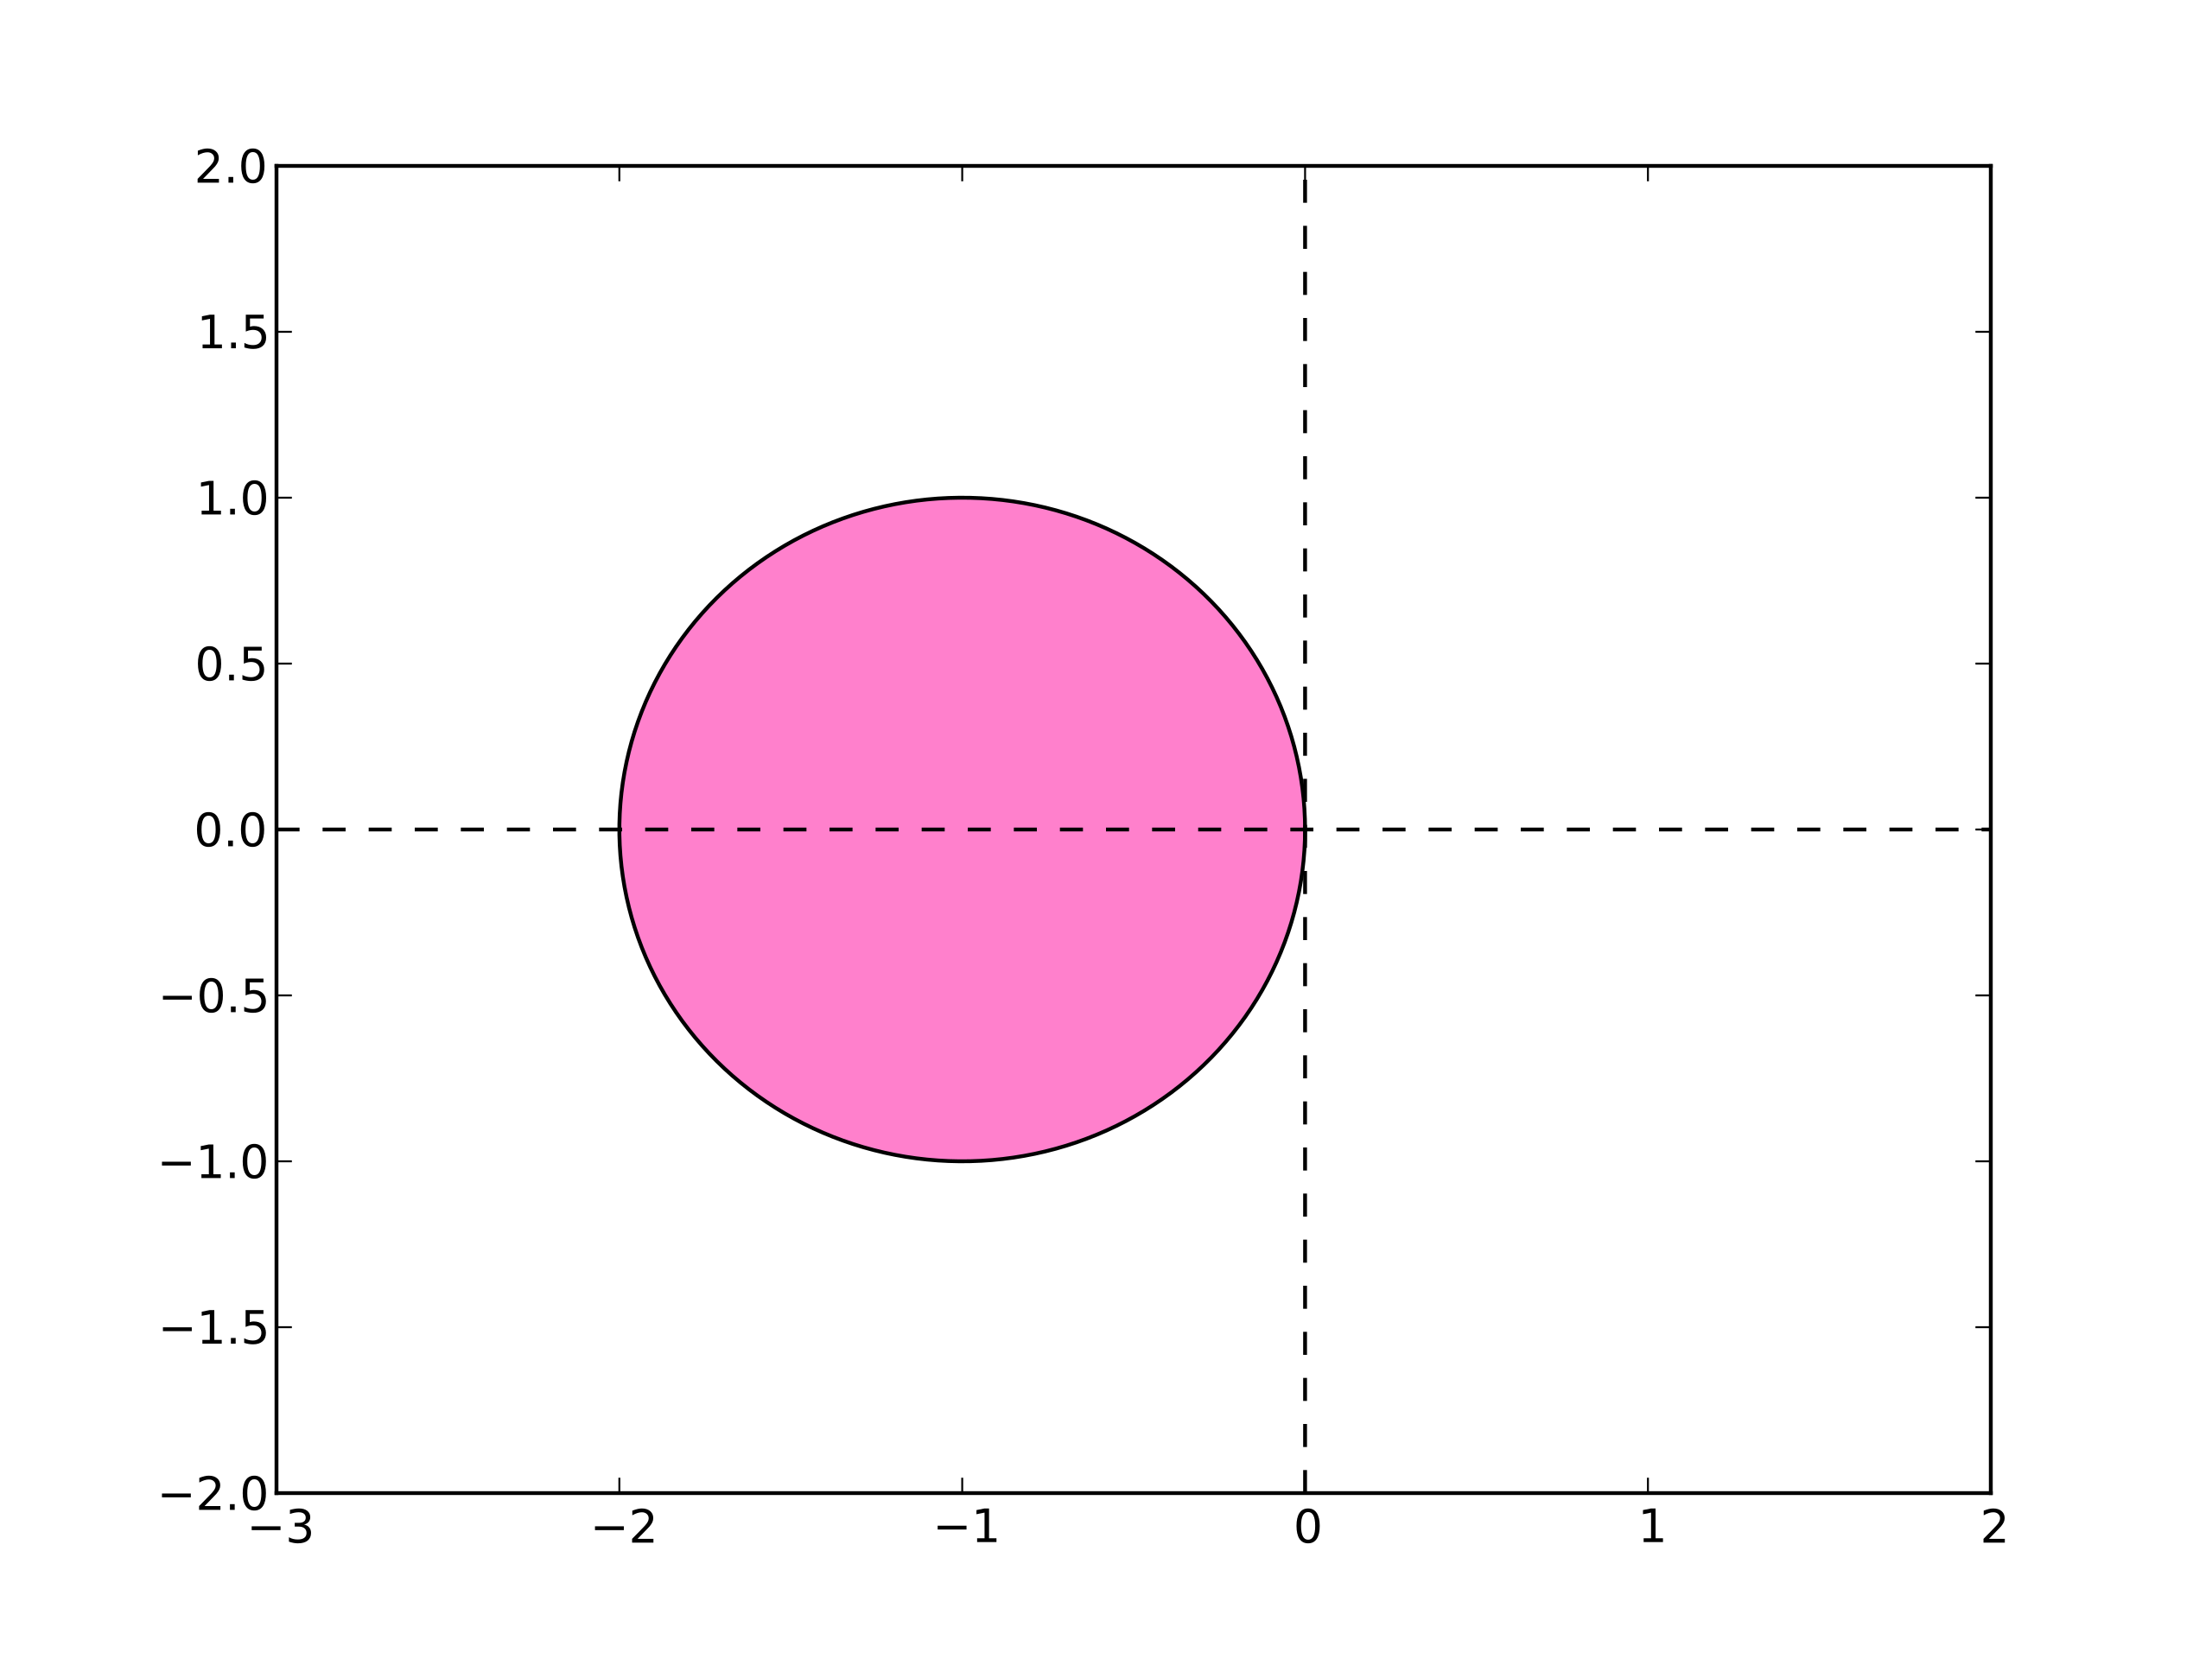
\includegraphics[width=0.7\textwidth]{FE_stability.png}
	\caption{The pink disk is the stability region for the Forward Euler method. This image is sourced from wikipedia.}
\end{figure}

\begin{constr}{Benchmark Problem}
.To find the region of stability, we use the benchmark problem
\begin{equation}
	y' = \lambda y
\end{equation}
whose solution is of the form $y = ce^{\lambda y}$.

$\lambda$ is some complex number.
\end{constr}

\subsubsection{Predictor-Corrector Method}

Yet another variation of this method is the following:

Instead of solving the implicit equation, we perform a certain iteration.

\begin{algo}{Predictor-Corrector Method}
.For example, suppose we want 4th order gloobal error.

Start with 4th order Adams-Bashford, getting 
\begin{equation}
	y_{n+1}^{(P)} \quad \text{(\textbf{prediction})}
\end{equation}

Next compute
\begin{equation}
	f(t_{n+1}, y_{n+1}^{(P)}) = f_{n+1}^{(E)} \quad \text{(\textbf{evaluated})}
\end{equation}

Next compute (using the Adams-Moulton method)
\begin{equation}
	y_{n+1}^{(C)} = y_n + \frac{h}{24}(9 f_{n+1}^{(E)} + 19 f_n - 5f_{n-1} + f_{n-2}) \quad \text{(\textbf{correction})}
\end{equation}
\end{algo}

This approach can be continued: we can
\begin{center}
	predict--evaluate--correct--(evaluate--correct)
\end{center}

And in principle we can keep evaluating and correcting as much as we want, but its often not advantageous to do so much more than twice.

\subsection{Stability}

Suppose the solution to the IVP (of dimension $n$) $y' = f(t, y)$ with some initial conditions is $y(t)$.

Let $\hat{y}(t)$ be the perturbation/a nearby function such that
\begin{equation}
	\hat{y}'(t) = f(t, \hat{y})
\end{equation}
with different initial conditions.

Consider the difference
\begin{equation}
	\omega(t) = y(t) - \hat{y}(t)
\end{equation}

We are interested in scenarios where as $t$ increases, this difference does not grow.

Consider the Taylor series expansion
\begin{equation}
	f(y) = f(\hat{y} + \omega) = f(\hat{y}) + \frac{\partial f}{\partial y} \omega + O(\lVert \omega \rVert^2)
\end{equation}
where
\begin{equation}
\frac{\partial f}{\partial y} = J_f = \begin{bmatrix}
	\nabla f_1^T \\
	\nabla f_2 ^T \\
	\vdots \\
	\nabla f_n ^T
\end{bmatrix}
\end{equation}
is the \textbf{Jacobian} (note from me: the Jacobian acts like a multi-dimensional/vector derivative).

Since $y' = f(y)$ and $\hat{y}' = f(\hat{y})$ (by definition), this Taylor expansion gives us the approximation
\begin{align}
	y' &= \hat{y}' + J_f \cdot \omega + O(\lVert \omega \rVert^2) \\
	y' &\approx \hat{y}' + J_f \cdot \omega
\end{align}

This suggests that the eigenvalues of $J_f$ influence the difference between $y'$and $\hat{y}'$.

This provides justification for our benchmarking problem $y' = \lambda y$.

\subsubsection{Example: 2nd Order Adams Bashford}

Consider the 2nd order Adams Bashford method
\begin{equation}
	y_{n+1} = y_n + \frac{h}{2}(3 f_n - f_{n-1})
\end{equation}

Apply our model problem
\begin{equation}
	y' = \lambda y
\end{equation}

We get
\begin{align}
	y_{n+1} &= y_n + \frac{h}{2}(3 \lambda y_n - \lambda y_{n-1}) \\
	&= \left( 1 + \frac{3h\lambda}{2} \right) y_n - \frac{h}{2} \lambda y_{n-1}
\end{align}

We claim:
\begin{equation}
	y(t_n) = e_n
\end{equation}

Plugging in this, we get
\begin{equation}
	e_{n+1} \approx \left( 1 + \frac{3h\lambda}{2} \right) e_n - \frac{h\lambda}{2}e_{n-1}
\end{equation}

So the errors approximately satisfy the 3-term recurrence relation
\begin{equation}
	e_{n+1} - \left( 1 + \frac{3h\lambda}{2} \right) e_n + \frac{h\lambda}{2}e_{n-1} = 0
\end{equation}

We solve this by guessing that the solution satisfies
\begin{equation}
	e_m = \rho^m
\end{equation}

Plugging this in, we get
\begin{equation}
	\rho^{m+1} - \left( 1 + \frac{3h\lambda}{2} \right) \rho^m + \frac{h\lambda}{2}\rho^{m-1} = 0
\end{equation}

Dividing by $\rho^{m-1}$ gives us
\begin{equation}
	\rho^2 - \left( 1 + \frac{3h\lambda}{2} \right) \rho + \frac{h\lambda}{2} = 0
\end{equation}

Which has solutions
\begin{equation}
	\rho = \frac{1}{2} \left( 1 + \frac{3h\lambda}{2} \pm \sqrt{\left( 1 + \frac{3h\lambda}{2} \right)^2 - 2h\lambda} \right)
\end{equation}

We want the error to decrease, that is we want
\begin{equation}
	\lvert \rho \rvert < 1
\end{equation}

$\lvert \rho \rvert < 1$ gives us the region of stability.

\begin{figure}[H]
	\centering
	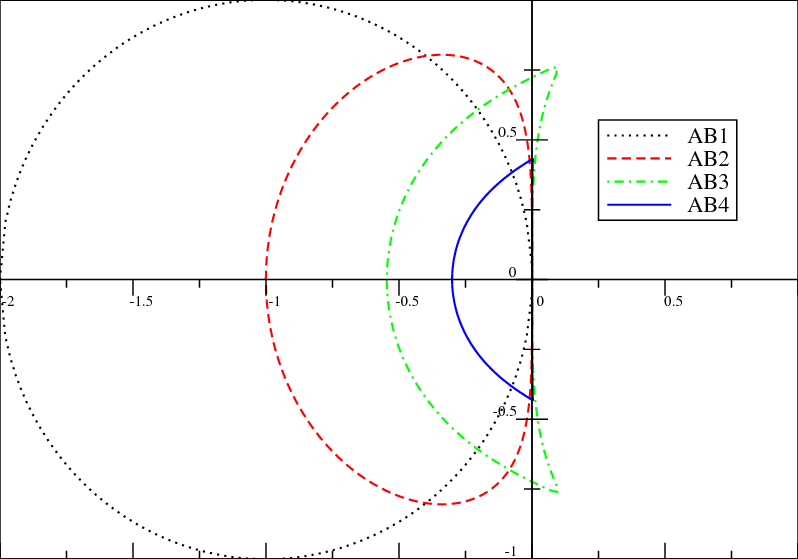
\includegraphics[width=0.7\textwidth]{AB_stability.png}
	\caption{The regions of stability for some Adams Bashford methods. Note that AB1 (1st order Adams Bashford) is the forward Euler method. Image sourced from \url{https://www.doi.org/10.12942/lrr-2009-1}.}
\end{figure}

\subsection{Stiff IVPs}

We consider the inital value problem $y' = f(t,y)$ as before.

Consider the Taylor expansion
\begin{equation}
	y(t_{n+1}) = y(t_n) + hy'(t_n) + \frac{h^2}{2} y''(\nu)
\end{equation}

We use our benchmarking problem
\begin{equation}
	y' = \lambda y
\end{equation}

Note that this implies
\begin{align}
	y &= ce^{\lambda t} \\
	y' &= c\lambda e^{\lambda t} \\
	y'' &= c\lambda^2 e^{\lambda t}
\end{align}

\textbf{Case 1:} Large $\lvert \lambda \rvert$.

To make LTE smaller than some tolerance $\tau$, we need
\begin{equation}
	\frac{h^2}{2} \lambda^2 e^{\lambda \nu} \leq \tau
\end{equation}

For example consider $\lambda=-100$, $\tau = 10^{-6}$. Then we would have
\begin{equation}
	\frac{h^2}{2}10^4 e^{-100} \leq 10^{-6}
\end{equation}
which requires approximately $h \leq 2\times10^{34}$. This is effectively no restriction.

Thus the stability bounds the time step. That is, this is a \textbf{stiff system}.

\textbf{Case 2:} Small $\lvert \lambda \rvert$.

Plug in for example $\lambda = -1$. We get
\begin{equation}
	\frac{h^2}{2} e^{-1} \leq 10^{-6}
\end{equation}
which yields the approximate bound $h \leq 10^{-3} \sqrt{2e}$.

In contrast, the stability bound is $h \leq \frac{2}{\lvert \lambda \rvert} = 2$, which is significantly larger.

Thus in this case the accuracy bounds the time step.

\begin{defn}{Stiff Systems}
.A system is called \textbf{stiff} when stability determines the time step size.
\end{defn}

\end{document}